% !TeX root = ../praktikum.tex
% !TeX encoding = UTF-8
% !Tex spellcheck = de_DE


Anhand der aufgenommenen Messdaten des Versuchsteils zur Winkelabhängigkeit wurde nun die Abhängigkeit des Quanten-Hall-Effekts, sowie des Shubnikov-de Haas-Effekts vom Einfallswinkel des Magnetfeldes auf die Probe analysiert.
Dazu wurden in Abbildung \ref{fig:winkel_ausw} die Magnetfeldwerte der Minima in Abhängigkeit des Winkels zur Probennormalen aufgetragen.
\begin{figure}[h]
	\centering
	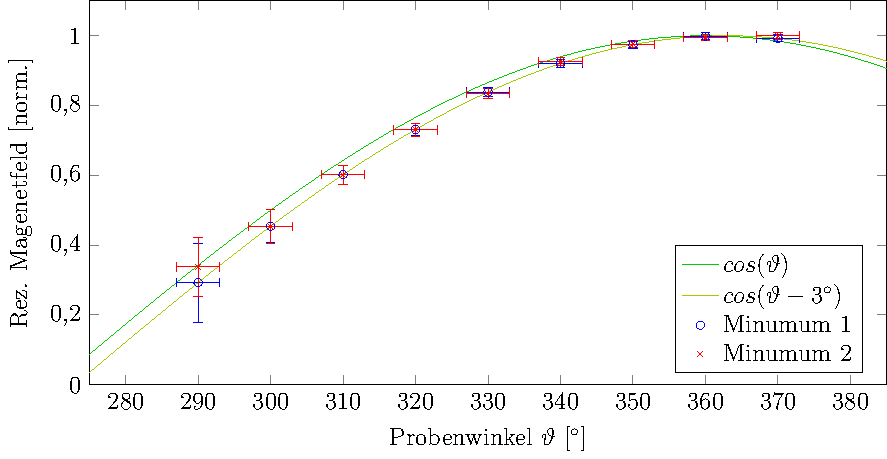
\includegraphics[scale=1]{graphs/winkel/auswertung.pdf}
	\caption[Auswertung der Winkelvariation]{
		Normierte Reziproke Magnetfelder zweier Minima der SDHO, aufgetragen gegen den Winkel der Probe zum Magnetfeld. Als Referenz sind zusätzlich zwei Cosinus-Funktionen hinzugefügt worden (s. Text).
	}
	\label{fig:winkel_ausw}
\end{figure}
Der hier angegebener Winkel von 360 beziehungsweise $370^\circ$ entspricht einer Auslenkung aus der Normalen der Probe zum Magnetfeld von 0 beziehungsweise $10^\circ$. In der Graphik wurden die Werte eines bestimmten Minimas bei unterschiedlichen Winkeleinstellungen gegen das reziproke Magnetfeld $\nicefrac{1}{B}$ aufgetragen. Zudem wurden hier die Positionen zweier verschiedener Minima (Minimum 1 mit einem Füllfaktor $\nu=16$ in rot, Minimum 2 mit $\nu=18$ in blau dargestellt) verglichen und um in einem Graphen vergleichbar dargestellt zu werden, auf den jeweils Maximalen Wert zu 1 normiert. 
Zwischen den Einstellungen 370 bis $320^{\circ}$ verläuft die Kurve Cosinusförmig. Bei Werten weiter links auf der x-Achse, welche hier einer größeren Auslenkung aus der Null-Position entsprechen, weicht die Kurve immer mehr von dieser Form ab. Für die Winkelabhängigkeit der beiden betrachteten Effekte wird theoretisch eine Cosinusfunktion erwartet, da bei einem Winkel von $0^{\circ}$ das effektive Magnetfeld am stärksten und bei einem Winkel von $90^{\circ}$ zur Probenfläche gleich Null ist. Ausgedrückt wird diese Beziehung durch das Skalarprodukt

\begin{equation}
	\vec{B} = \abs{\vec{B}} \cdot cos(\vartheta)
	\label{eq:winkelabh_skalarprodukt}
\end{equation}

Mit dem Winkel $\vartheta$ zwischen Magnetfeldlinien und Probennormalen. Die Ablesegenauigkeit des Probenwinkels wird auf$\pm 3 $ Grad geschätzt. Der Fehler in der Magnetfeldmessung wird auf $\pm \unit[0,01]{T}$ geschätzt. %Aufgrund des reziproken Auftragens des Magnetfeldes auf der y-Achse sind deren einzelne Fehler der Messpunkte um einen Faktor von bis zu $10^{-5}$ kleiner als die y-Werte selbst und wurden daher nicht im Graphen dargestellt.
Zur Anschauung sind die beiden Kurven der Funktionen $cos(\nu)$ und $cos(\nu-3^{\circ})$ zusammen mit den Messwerten in Abbildung~\ref{fig:winkel_ausw} aufgetragen. Es ist gut zu erkennen, dass die Kurve der Funktion $cos(\nu-3^{\circ})$ näher an den aus den Messdaten erhaltenen Werten liegt. Dies legt nahe, dass ein leichtes Offset vorliegt. Dieses könnte beispielsweise durch ein ungenaues Anbringen der (aufgeklebten Papier-)Winkelscheibe liegen.

Die hier dargestellte Abhängigkeit zeigt deutlich, dass für zunehmende Auslenkung aus der Nullposition höhere Magnetfelder, also kleinere Werte für $\nicefrac{1}{B}$ notwendig sind, um für die SDH-Oszillation Minima zu erzeugen und es kann angenommen werden, dass diese bei einer Auslenkung von 90 Grad vollständig verschwinden. 

